\section{ベイズ脳仮説と神経活動による不確実性の表現}

\subsection{ベイズ脳仮説}
Knill, David C., and Alexandre Pouget. 2004. “The Bayesian Brain: The Role of Uncertainty in Neural Coding and Computation.” Trends in Neurosciences 27 (12): 712–19.

\subsection{神経活動による不確実性の表現}
ここまでは最尤推定やMAP推定などにより,パラメータ(神経活動,シナプス結合)の点推定を行ってきた.\textbf{不確実性(uncertainty)} を神経回路で表現する方法として主に2つの符号化方法,\textbf{サンプリングに基づく符号化(sampling-based coding; SBC or neural sampling model)} および\textbf{確率的集団符号化(probabilistic population coding; PPC)} が提案されている.SBCは神経活動が元の確率分布のサンプルを表現しており,時間的に多数の活動を集めることで元の分布の情報が得られるというモデルである.PPCは神経細胞集団により,確率分布を表現するというモデルである.

\begin{itemize}
\item (Walker et al., 2022)がまとめ.
\item (Fiser et al., 2010)の比較表を入れる.
\item 神経活動の変動性 (neural variability)
\item 自発活動が事前分布であるという説 \cite{Fiser2010-kw}, \cite{Berkes2011-it}.
\item \cite{Hoyer2002-ci}
\item \cite{Sanborn2016-en}
\end{itemize}
\lstinputlisting[language=julia]{./text/bayesian-brain/neural-uncertainty-representation/001.jl}
\begin{figure}[ht]
	\centering
	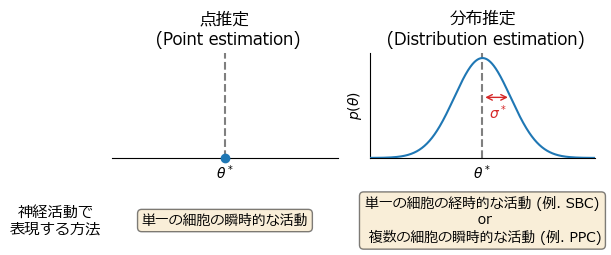
\includegraphics[scale=0.8, max width=\linewidth]{./fig/bayesian-brain/neural-uncertainty-representation/cell001.png}
	\caption{cell001.png}
	\label{cell001.png}
\end{figure}
\lstinputlisting[language=julia]{./text/bayesian-brain/neural-uncertainty-representation/002.jl}
\lstinputlisting[language=julia]{./text/bayesian-brain/neural-uncertainty-representation/003.jl}
\begin{figure}[ht]
	\centering
	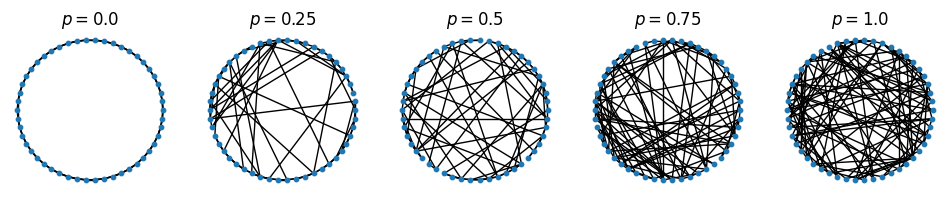
\includegraphics[scale=0.8, max width=\linewidth]{./fig/appendix/graph-theory-network-model/cell003.png}
	\caption{cell003.png}
	\label{cell003.png}
\end{figure}
